\section{Lefschetz 对偶}
\sourcepage{497--498}
正如预期，Poincaré 对偶可推广到相对同调流形，这一推广归功于 Lefschetz。在流形情形，它具有特别漂亮的形式。

先回顾：若 $X$ 中任意顶点全在 $A$ 的单形都属于 $A$，就称 $A$ 为\emph{满子复形}。一般子复形不一定满，但重心重分后总成为满子复形。事实上，若重分单形的顶点均在 $\operatorname{sd}A$ 中，特别是最大顶点 $\widehat\sigma_1$ 在其中，则 $\Int\sigma_1$ 与 $|A|$ 相交，故 $\sigma_1\in A$，整个重分单形也在 $|A|$ 中。

\entry{引理}{8.10.1}设 $A$ 为有限复形 $X$ 的满子复形，$C$ 由所有与 $|A|$ 不交的单形组成。则 $|A|$ 是 $|X|\setminus|C|$ 的形变收缩核，$|C|$ 是 $|X|\setminus|A|$ 的形变收缩核。

\textbf{证明：}每个顶点属于 $A$ 或 $C$。$C$ 也是满子复形：顶点都在 $C$ 的单形不可能与 $|A|$ 相交。反过来，$A$ 也恰由所有与 $|C|$ 不交的单形组成，因为这样的单形顶点都在 $A$ 中。由对称性只证第一个结论。

若 $\sigma$ 既不属于 $A$ 也不属于 $C$，则 $\sigma=s*t$，其中 $s$ 由属于 $A$ 的顶点张成，$t$ 由属于 $C$ 的顶点张成。每个 $x\in\sigma\setminus(s\cup t)$ 都在连接两部分的唯一线段内部。令 $f_\sigma(x)$ 为该线段在 $s$ 一侧的端点，并在 $s$ 上取恒等。若 $s=v_0\cdots v_p$、$t=v_{p+1}\cdots v_r$，则
\[x=\sum_{i=0}^r\alpha_iv_i\quad\Longrightarrow\quad
f_\sigma(x)=\sum_{i=0}^p\frac{\alpha_i}{\lambda}v_i,\qquad\lambda=\sum_{i=0}^p\alpha_i>0.\]
所以 $f_\sigma$ 连续。这些映射在公共部分相容，且在 $|A|$ 上为恒等，因此拼成收缩 $f:|X|\setminus|C|\to|A|$。令 $F(x,t)=(1-t)x+tf(x)$，即为所需形变收缩。\hfill$\square$

引理在无限复形情形也成立，但连续性需要额外注意；有限情形没有这个问题。

\entry{定义}{8.10.2}设 $(X,A)$ 为紧致、已三角剖分的相对同调 $n$ 维流形。若能给所有不属于 $A$ 的顶维单形定向，使其和 $\gamma$ 为相对闭链，则称该偶\emph{可定向}，称 $\gamma$ 为\emph{定向闭链}。

\entry{定理}{8.10.3（Lefschetz 对偶）}若 $(X,A)$ 紧致、已三角剖分，且是可定向的相对同调 $n$ 维流形，则对任意 $G$，
\[H^k(X,A;G)\cong H_{n-k}(|X|\setminus|A|;G),\qquad
H_k(X,A;G)\cong H^{n-k}(|X|\setminus|A|;G).\]
若不可定向，取 $G=\Z/2$ 时仍成立。

\entry{注}{8.10.4}补空间的群应理解为奇异群，因为它不是原复形子复形的多面体（它实际上可三角剖分，但还未证明）。

\textbf{证明：}令 $X^*$ 为 $\operatorname{sd}X$ 中所有与 $|A|$ 不交的单形组成的子复形。$\operatorname{sd}A$ 满，故由引理 $|X^*|$ 是补空间的形变收缩核，可用它代替补空间。

\sourcepage{499}
断言：$|X^*|$ 等于所有不属于 $A$ 的单形所对应对偶块之并。若重分单形对应面链 $\sigma_1\succ\cdots\succ\sigma_k$，其内部属于 $D(\sigma_k)$。它与 $|A|$ 不交，当且仅当 $\sigma_k\notin A$：一个方向看最小顶点即可；反方向，若最小单形不在 $A$ 中，所有包含它的较大单形也不在 $A$ 中，故各重心均不在 $A$ 中，整个重分单形不与 $|A|$ 相交。

\begin{figure}[htbp]\centering
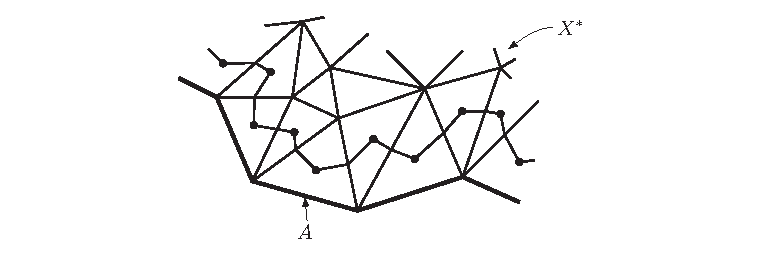
\includegraphics[width=.90\textwidth]{figures/8-10-1.pdf}
\caption*{图 8.10.1}
\end{figure}

这些块的重心位于 $X\setminus A$，局部同调满足流形条件，所以每个闭块模边界是维数 $n-\dim\sigma$ 的同调胞腔。它们组成对偶链复形 $\mathcal D(X^*)$，其包含到 $C(X^*)$ 的映射诱导任意系数的同调、上同调同构，理由同定理 8.4.8。

可定向情形，$C^k(X,A)$ 是在 $A$ 的单形上为零的上链群，其基由所有 $\sigma\notin A$ 的 $\sigma^*$ 构成。第一种 Poincaré 对偶证明原样给出
\[\varphi:C^k(X,A)\xrightarrow{\cong}\mathcal D_{n-k}(X^*),\qquad\varphi\delta=\partial\varphi.\]
于是得到第一个对偶同构。

\sourcepage{500}
有限自由链群的自然双对偶同构把 $\operatorname{Hom}(C^k(X,A),\Z)$ 与 $C_k(X,A)$ 等同。再将 $\varphi$ 对偶化，就得到相对同调与对偶复形上同调的同构，进而得到第二个对偶同构。任意系数以及不可定向时的模 $2$ 情形，与 Poincaré 对偶证明相同。\hfill$\square$

\entry{推论}{8.10.5}若补空间连通，则任意两个不属于 $A$ 的顶维单形之间，都有相邻单形交于不属于 $A$ 的余维一面的有限顶维单形序列。

\textbf{证明：}以这种序列定义等价关系。每个等价类之和均为模 $2$ 相对闭链，而
\[H_n(X,A;\Z/2)\cong H^0(|X|\setminus|A|;\Z/2)\cong\Z/2,\]
所以只有一个等价类。\hfill$\square$

\entry{推论}{8.10.6}若补空间连通，则可定向时 $H_n(X,A)\cong\Z$，不可定向时 $H_n(X,A)=0$。

证明同推论 8.5.4。

\sourcepage{501}
\entry{推论}{8.10.7}令 $X_i$ 为补空间各连通分支的闭包，$A_i=X_i\cap A$。则 $(X,A)$ 可定向，当且仅当每个 $H_n(X_i,A_i)\cong\Z$。

\entry{注}{8.10.8}因此相对可定向性与三角剖分无关。

\entry{定义}{8.10.9}设 $(X,A)$ 为紧致、可三角剖分的相对同调 $n$ 维流形。采用上一推论的记号。可定向时，选取每个 $H_n(X_i,A_i)$ 的生成元 $\Gamma^{(i)}$，称为该偶的定向类；它们的和通过包含诱导同构
\[\bigoplus_i H_n(X_i,A_i)\cong H_n(X,A)\]
的像称为 $(X,A)$ 的\emph{定向类}，记为 $\Gamma$。不要求可定向时，取各模 $2$ 顶维相对同调的唯一非零元，其和记为 $\Gamma_{(2)}$。若给定剖分，分别由适当定向的全部不属于 $A$ 的顶维单形之和，或这些单形均取系数 $[1]$ 的和代表。

自然会问：帽积形式的第二种证明能否直接推广？一般不能。选恒等映射的单纯逼近 $g:(\operatorname{sd}X,\operatorname{sd}A)\to(X,A)$，以及定向相对闭链 $\gamma$。前面的论证仍表明复合
\[C^k(X,A)\xrightarrow{g^\#}C^k(\operatorname{sd}X,\operatorname{sd}A)
\xrightarrow{\frown\operatorname{sd}\gamma}C_{n-k}(\operatorname{sd}X)\]
同构地映到对偶链子群 $\mathcal D_{n-k}(X^*)$，并与 $\varphi$ 仅差一个符号。

\sourcepage{502}
困难发生在通过同调时：帽积的目标是 $H_{n-k}(X)$，而不是所需的 $H_{n-k}(X\setminus A)$。因此一般不能直接把 Lefschetz 对偶同构写成与 $\Gamma$ 的帽积，只能得到如下关系。

\entry{定理}{8.10.10}令 $j:X\setminus A\to X$ 为包含，$\varphi_*$ 为 Lefschetz 对偶同构。则对可定向的紧致可三角剖分相对同调流形，
\[\frown\Gamma=\pm j_*\varphi_*:H^k(X,A;G)\to H_{n-k}(X;G),\]
符号只依赖 $k,n$。不可定向情形以 $\Gamma_{(2)}$ 和 $\Z/2$ 代替，结论同样成立。

\textbf{证明：}选取剖分，比较 $\varphi$ 与上述重分后帽积复合。第 8.7 节的证明说明二者相差维数相关的符号。再将对偶链包含到 $X^*$ 的单纯链，映到奇异链，并由包含映入补空间及 $X$；单纯到奇异的链映射保持帽积，其余包含映射显然交换。通过同调即得结论。\hfill$\square$

对带边界流形，对偶同构确实可以由帽积直接给出。

\sourcepage{503--504}
\entry{定义}{8.10.11}若有同胚 $h:\Bd M\times[0,1)\to U$，其中 $U$ 是 $M$ 中开集，且 $h(x,0)=x$，则称边界在 $M$ 中有\emph{乘积邻域}。这样的邻域实际上总存在，但证明并不简单（见 [Bro62]）。

\entry{定理}{8.10.12（Poincaré--Lefschetz 对偶）}设 $M$ 是紧致、可三角剖分的带边界 $n$ 维流形，边界有乘积邻域。若 $(M,\Bd M)$ 可定向，取定向类 $\Gamma$，则对任意 $G$，
\[H^k(M,\Bd M;G)\xrightarrow{\frown\Gamma}H_{n-k}(M;G),\]
\[H^k(M;G)\xrightarrow{\frown\Gamma}H_{n-k}(M,\Bd M;G)\]
都是同构。不可定向时，取 $\Z/2$ 系数与 $\Gamma_{(2)}$ 也成立。

\begin{figure}[htbp]\centering
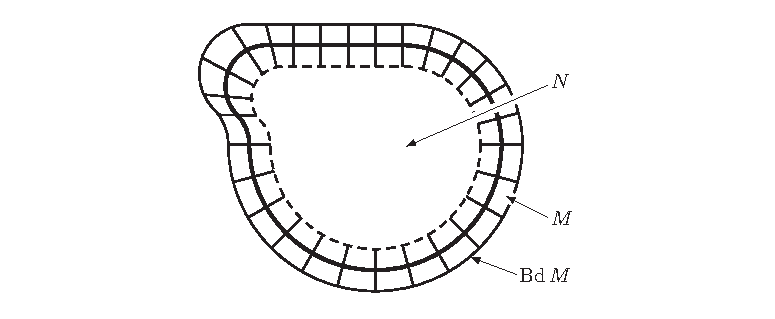
\includegraphics[width=.90\textwidth]{figures/8-10-2.pdf}
\caption*{图 8.10.2}
\end{figure}

\textbf{证明：}取边界乘积邻域 $h$，令
\[N=M\setminus h(\Bd M\times[0,1/2)).\]
将乘积参数向 $1/2$ 推动，表明 $N$ 同时是 $M$ 与 $M\setminus\Bd M$ 的形变收缩核。因此内部到 $M$ 的包含为同伦等价，诱导同调同构。第一个帽积同构随即由定理 8.10.10 得到。

证明第二个。三角剖分边界是 $(n-1)$ 维单形之并，每个边界余维一面恰为一个顶维单形的面：至少有一个，因为 $M$ 由顶维单形组成；不能多于一个，因为边界点的局部同调为零，而引理 8.3.2 把该局部群与链环的约化零维同调等同。

若 $\gamma$ 是相对定向闭链，则 $\partial\gamma$ 在每个边界顶维单形上系数均为 $\pm1$，且为闭链，所以是边界的定向闭链。故 $\partial_*\Gamma$ 是 $\Bd M$ 的定向类。比较偶的上同调、同调长正合列中的五项，对应竖直映射依次为
\[\frown\partial_*\Gamma,\quad\frown\Gamma,\quad\frown\Gamma,\quad
\frown\partial_*\Gamma,\quad\frown\Gamma.\]
源的五项依次为 $H^{k-1}(\Bd M),H^k(M,\Bd M),H^k(M),H^k(\Bd M),H^{k+1}(M,\Bd M)$；目标为相应的 $H_{n-k}(\Bd M),H_{n-k}(M),H_{n-k}(M,\Bd M),H_{n-k-1}(\Bd M),H_{n-k-1}(M)$。图相差符号地交换。第一、四项由 Poincaré 对偶为同构，第二、五项由刚证明的第一个同构为同构，因此五引理给出中间项同构。模 $2$ 时证明相同。\hfill$\square$

给定紧致流形，什么时候它是某个高一维紧致流形的边界？研究这一问题的完整理论称为\emph{配边理论}。下面只证明一个初等结果。

\sourcepage{505--506}
\entry{定理}{8.10.13}设 $M$ 是紧致、可三角剖分的带边界 $(2m+1)$ 维流形，边界非空且有乘积邻域。则 $H_m(\Bd M;\Z/2)$ 的维数为偶数。

\textbf{证明：}第一步：对只在有限范围非零的向量空间正合列 $\cdots\to A_{k-1}\xrightarrow{\varphi_{k-1}}A_k\xrightarrow{\varphi_k}A_{k+1}\to\cdots$，有
\[
\operatorname{rank}\varphi_k=\dim A_k-\dim A_{k-1}+\dim A_{k-2}-\cdots,
\]
\[
\operatorname{rank}\varphi_{k-1}=\dim A_k-\dim A_{k+1}+\dim A_{k+2}-\cdots.
\]
因为正合性给出 $\dim A_i=\operatorname{rank}\varphi_{i-1}+\operatorname{rank}\varphi_i$，交错求和即可。

第二步：取模 $2$ 上同调长正合列中的映射
\[H^k(M)\xrightarrow{\mu_k}H^k(\Bd M)\xrightarrow{\nu_k}H^{k+1}(M,\Bd M).\]
记三类群的维数分别为 $\beta_k,\gamma_k,\alpha_{k+1}$。第一步给出
\[\operatorname{rank}\nu_k=\sum_{i\ge0}(-1)^i(\gamma_{k-i}-\beta_{k-i}+\alpha_{k-i}),\]
\[\operatorname{rank}\mu_k=\sum_{i\ge0}(-1)^i(\gamma_{k+i}-\alpha_{k+i+1}+\beta_{k+i+1}).\]
令 $n=\dim M$。Lefschetz 对偶、边界上的 Poincaré 对偶以及域系数代数对偶给出
\[\alpha_j=\beta_{n-j},\qquad\gamma_j=\gamma_{n-j-1}.\]
代入比较两式，得 $\operatorname{rank}\mu_k=\operatorname{rank}\nu_{n-k-1}$。当 $n=2m+1$ 时，$\operatorname{rank}\mu_m=\operatorname{rank}\nu_m$，所以
\[\dim H_m(\Bd M;\Z/2)=\gamma_m=2\operatorname{rank}\nu_m,\]
为偶数。\hfill$\square$

\entry{推论}{8.10.14}$P^{2m}$ 不是紧致、可三角剖分的 $(2m+1)$ 维流形的边界。

\subsection*{习题}
\begin{enumerate}
\item 设 $(X,A)$ 是紧致、可三角剖分的相对同调 $n$ 维流形，补空间连通。证明可定向时
\[H_n(X,A;G)\cong G\cong H^n(X,A;G),\]
不可定向时
\[H_n(X,A;G)\cong\ker\varphi_2,\qquad H^n(X,A;G)\cong G/2G,\]
其中 $\varphi_2$ 为乘以 $2$。
\item 设 $M$ 是紧致可定向、可三角剖分的带边界 $n$ 维流形，边界为两个 $(n-1)$ 维流形 $V_0,V_1$ 的不交并，且有乘积邻域。取相对定向类 $\Gamma$，证明
\[\frown\Gamma:H^k(M,V_0)\longrightarrow H_{n-k}(M,V_1)\]
为同构。〔提示：考虑三元组 $(M,\Bd M,V_1)$ 的正合列。〕
\item 利用复射影空间可三角剖分，证明 $\mathbb{CP}^{2m}$ 不是任何流形的边界。
\item 哪些紧致二维流形能够成为边界？
\item 设 $M$ 为紧致可定向、可三角剖分的带边界 $n$ 维流形。证明杯积给出对偶配对
\[\frac{H^k(M,\Bd M)}{T^k(M,\Bd M)}\otimes
\frac{H^{n-k}(M)}{T^{n-k}(M)}\to H^n(M,\Bd M),\]
其中 $T^i$ 表示相应上同调群的挠子群。
\item 设 $M$ 是从环面删去两个开圆盘所得的空间（图 8.10.3）。
\begin{enumerate}[label=(\alph*)]
\item 计算 $H^1(M)$、$H^1(M,\Bd M)$，画出生成上闭链。
\item 验证上一题的对偶配对。
\item 证明两个相对一维上同调因子的杯积
\[\frac{H^1(M,\Bd M)}{T^1(M,\Bd M)}\otimes
\frac{H^1(M,\Bd M)}{T^1(M,\Bd M)}\to H^2(M,\Bd M)\]
并不构成对偶配对。
\end{enumerate}
\begin{figure}[htbp]\centering

\includegraphics[width=.90\textwidth]{figures/8-10-3.pdf}
\caption*{图 8.10.3}
\end{figure}
\item 设 $X$ 为紧致、可三角剖分的同调 $n$ 维流形，$B\subset A$ 均为同一剖分的子复形多面体。可定向时 $G$ 任意，否则取 $G=\Z/2$。证明
\[H^k(A,B;G)\cong H_{n-k}(X\setminus B,X\setminus A;G),\]
\[H_k(A,B;G)\cong H^{n-k}(X\setminus B,X\setminus A;G).\]
〔提示：选择剖分使 $A,B$ 均为满子复形的多面体。对满子复形 $C$，记 $X_C$ 为重分后与 $C$ 不交的全部单形组成的复形。比较上链短正合列
\[0\to C^k(X,A)\to C^k(X,B)\to C^k(A,B)\to0\]
与对偶链短正合列
\[0\to\mathcal D_{n-k}(X_A)\to\mathcal D_{n-k}(X_B)
\to\mathcal D_{n-k}(X_B,X_A)\to0,\]
以及它们的对偶。〕
\item 〔*〕将 Lefschetz 对偶推广到非紧情形。
\item 设 $(X,A)$ 为非紧的已三角剖分相对同调 $n$ 维流形，且补空间连通。证明它是相对伪 $n$ 维流形。
\item 给出两个二维的紧致可三角剖分相对同调流形例子，并分别指定定向类。
\end{enumerate}
